\section{Polychromatic Correction Temperature Fit Residual Data Plots}
%=====================================================================
\label{app.tfit_data_plots}
%\newpage

\subsection{Imager}
%------------------

\begin{figure}[H]
  \centering
  \begin{tabular}{c c}
    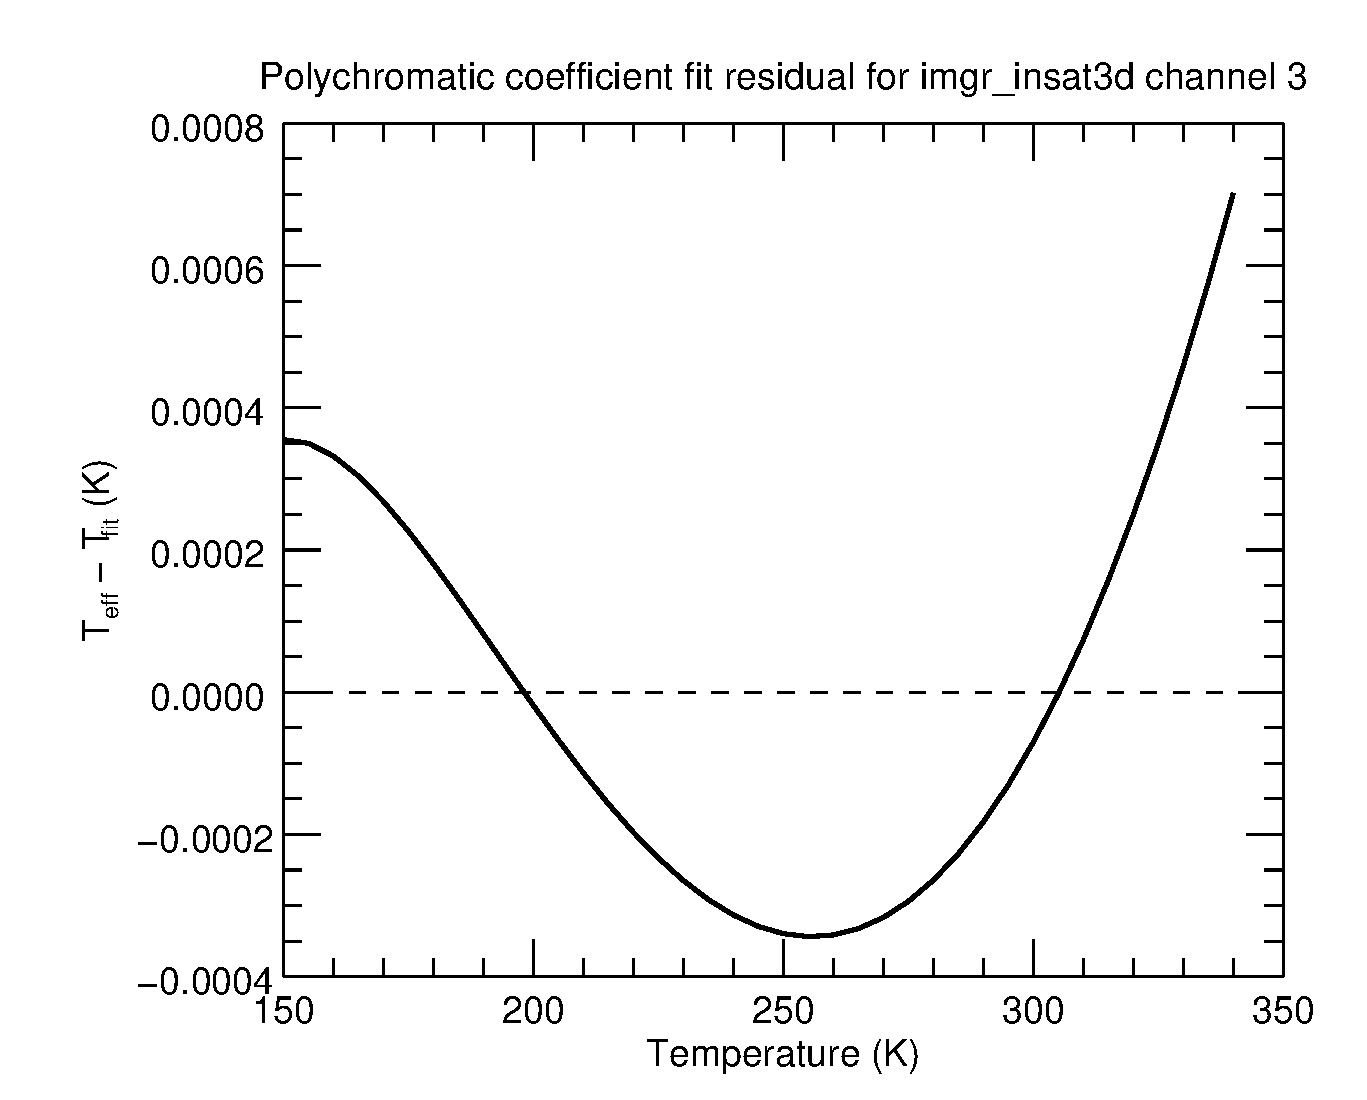
\includegraphics[scale=0.35]{graphics/imgr/tfit/imgr_insat3d-3.tfit.eps} &
    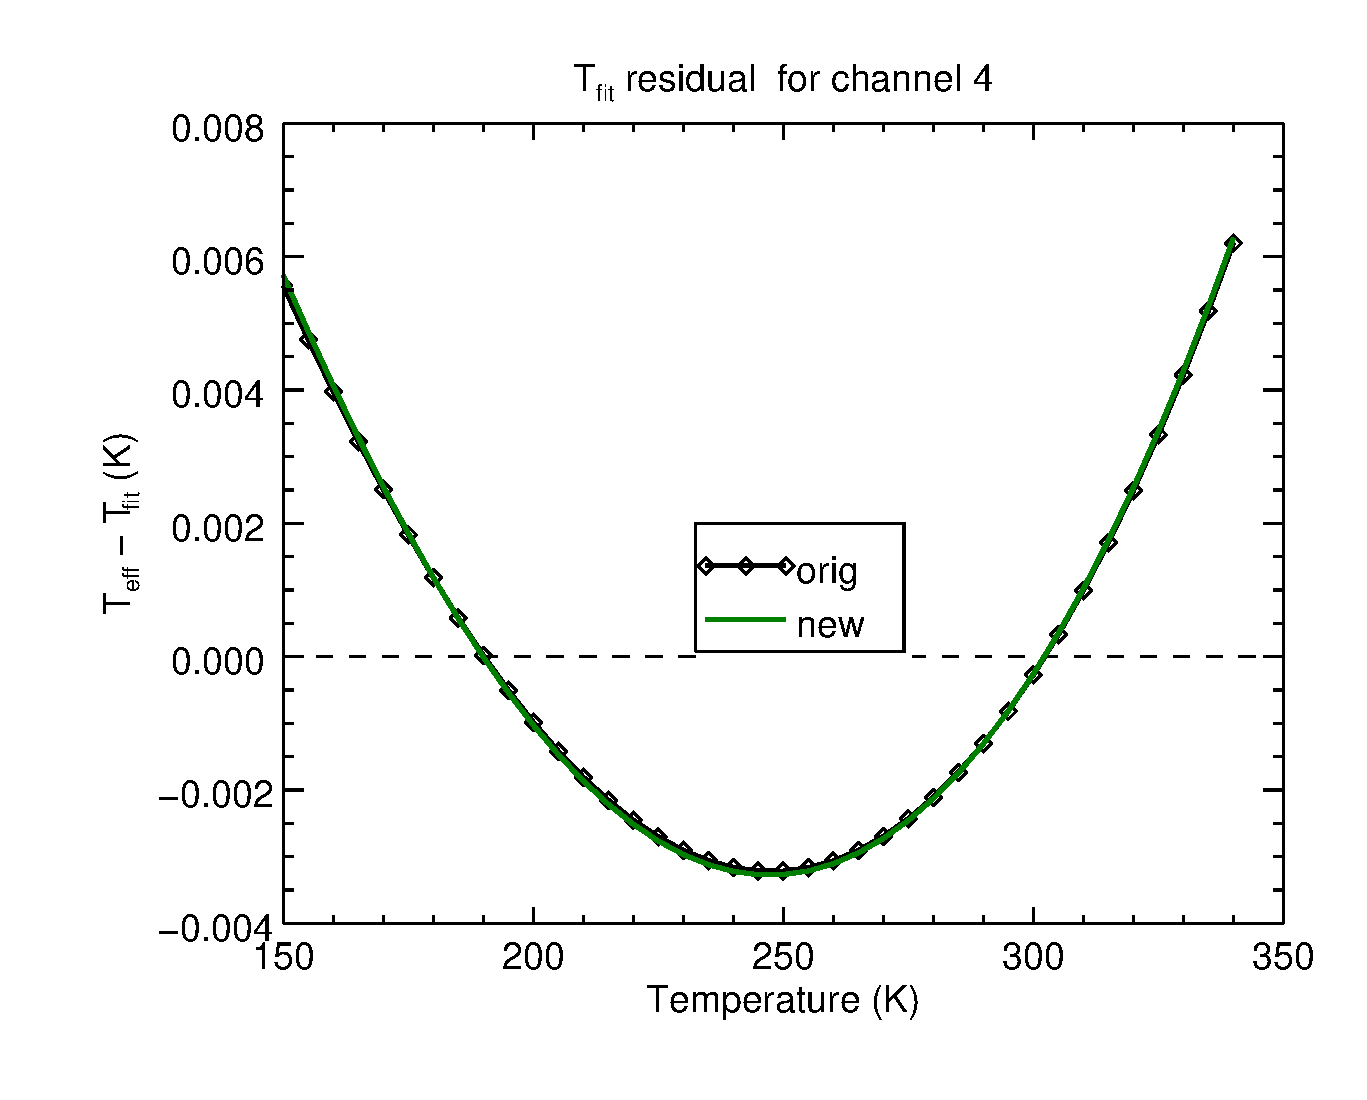
\includegraphics[scale=0.35]{graphics/imgr/tfit/imgr_insat3d-4.tfit.eps} \\\\
    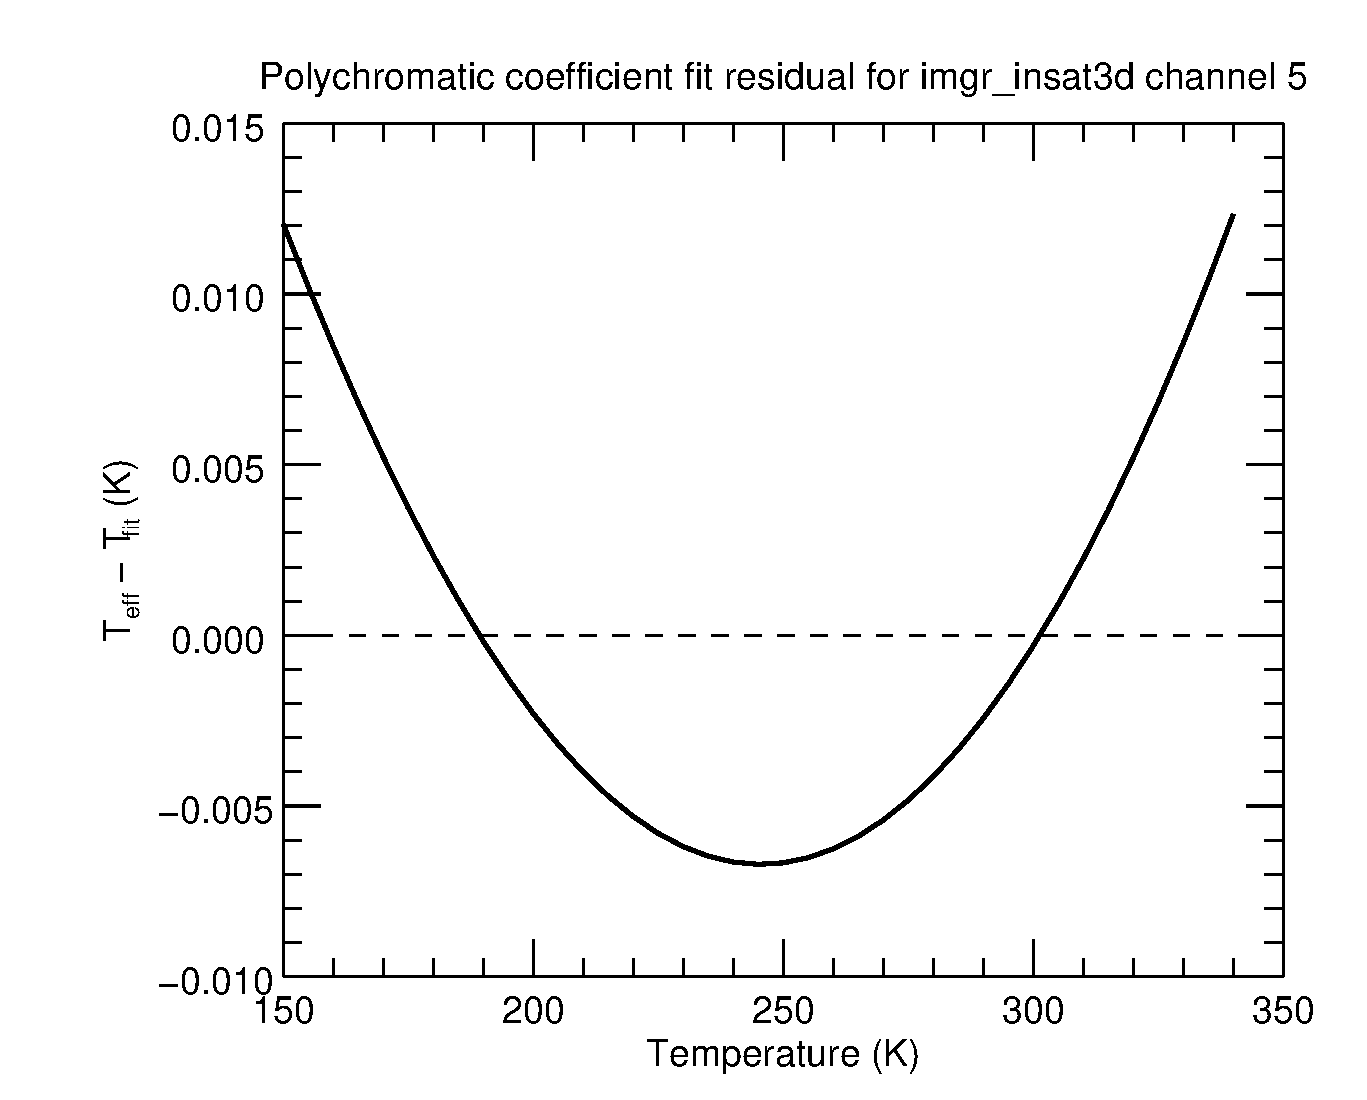
\includegraphics[scale=0.35]{graphics/imgr/tfit/imgr_insat3d-5.tfit.eps} &
    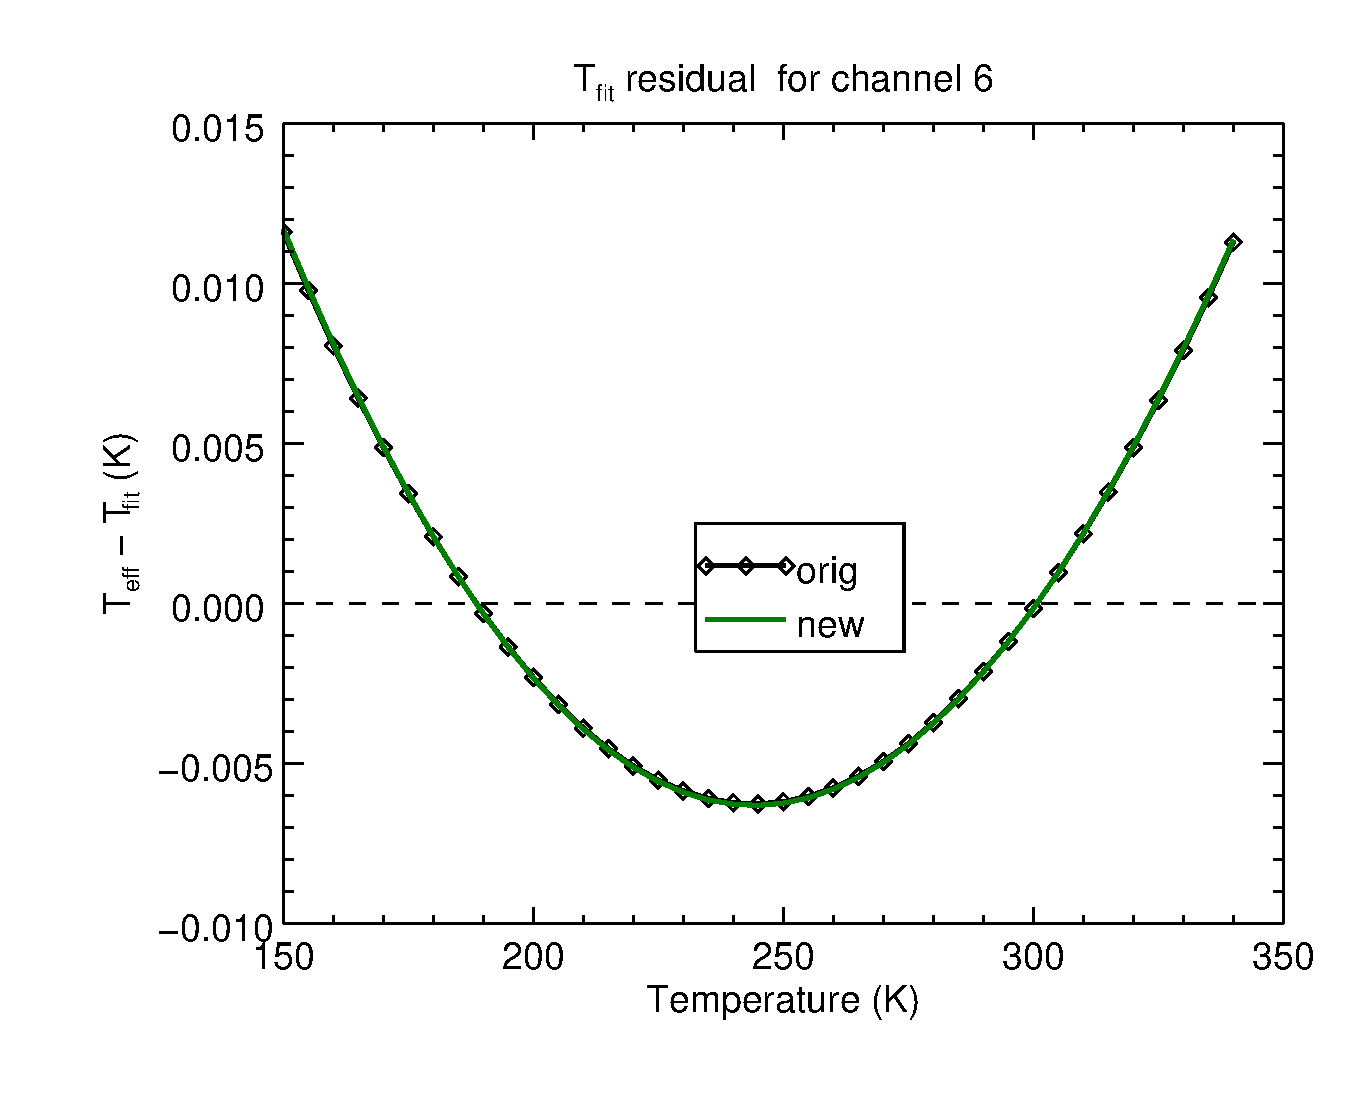
\includegraphics[scale=0.35]{graphics/imgr/tfit/imgr_insat3d-6.tfit.eps} \\
  \end{tabular}
  \caption{INSAT-3D Imager channels 3-6 polychromatic correction temperature fit residuals.}
  \label{fig:imgr_ch1-6_tfit}
\end{figure}

\subsection{Sounder}
%------------------

\addcontentsline{toc}{subsubsection}{Channels 1-6}
\begin{figure}[H]
  \centering
  \begin{tabular}{c c}
    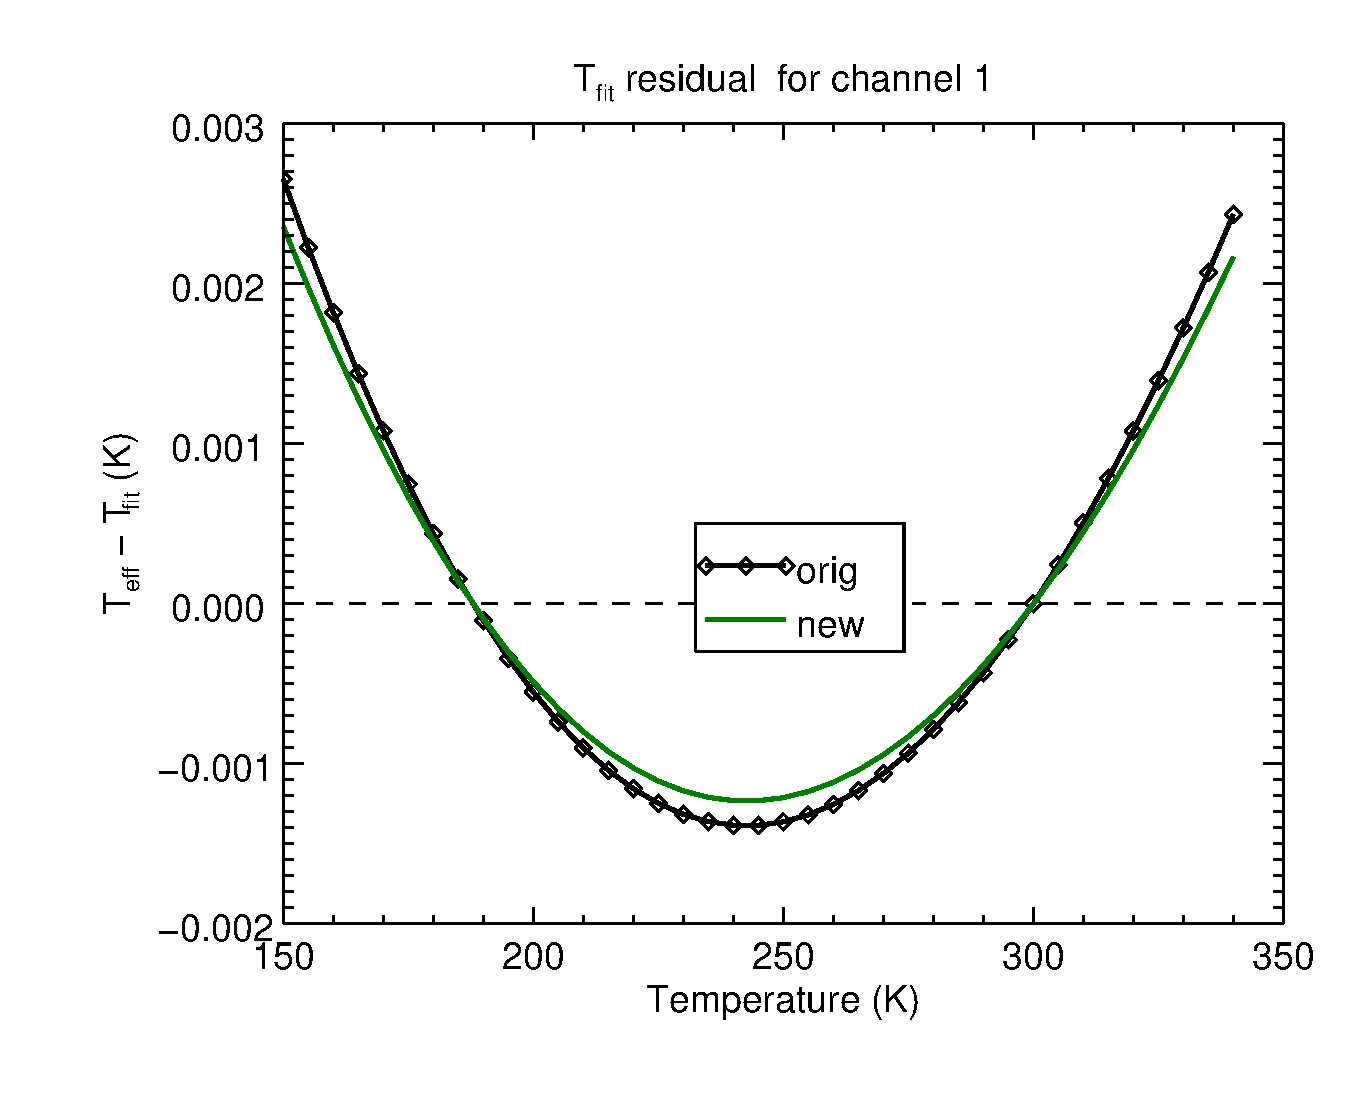
\includegraphics[scale=0.35]{graphics/sndr/tfit/sndr_insat3d-1.tfit.eps} &
    \includegraphics[scale=0.35]{graphics/sndr/tfit/sndr_insat3d-2.tfit.eps} \\\\
    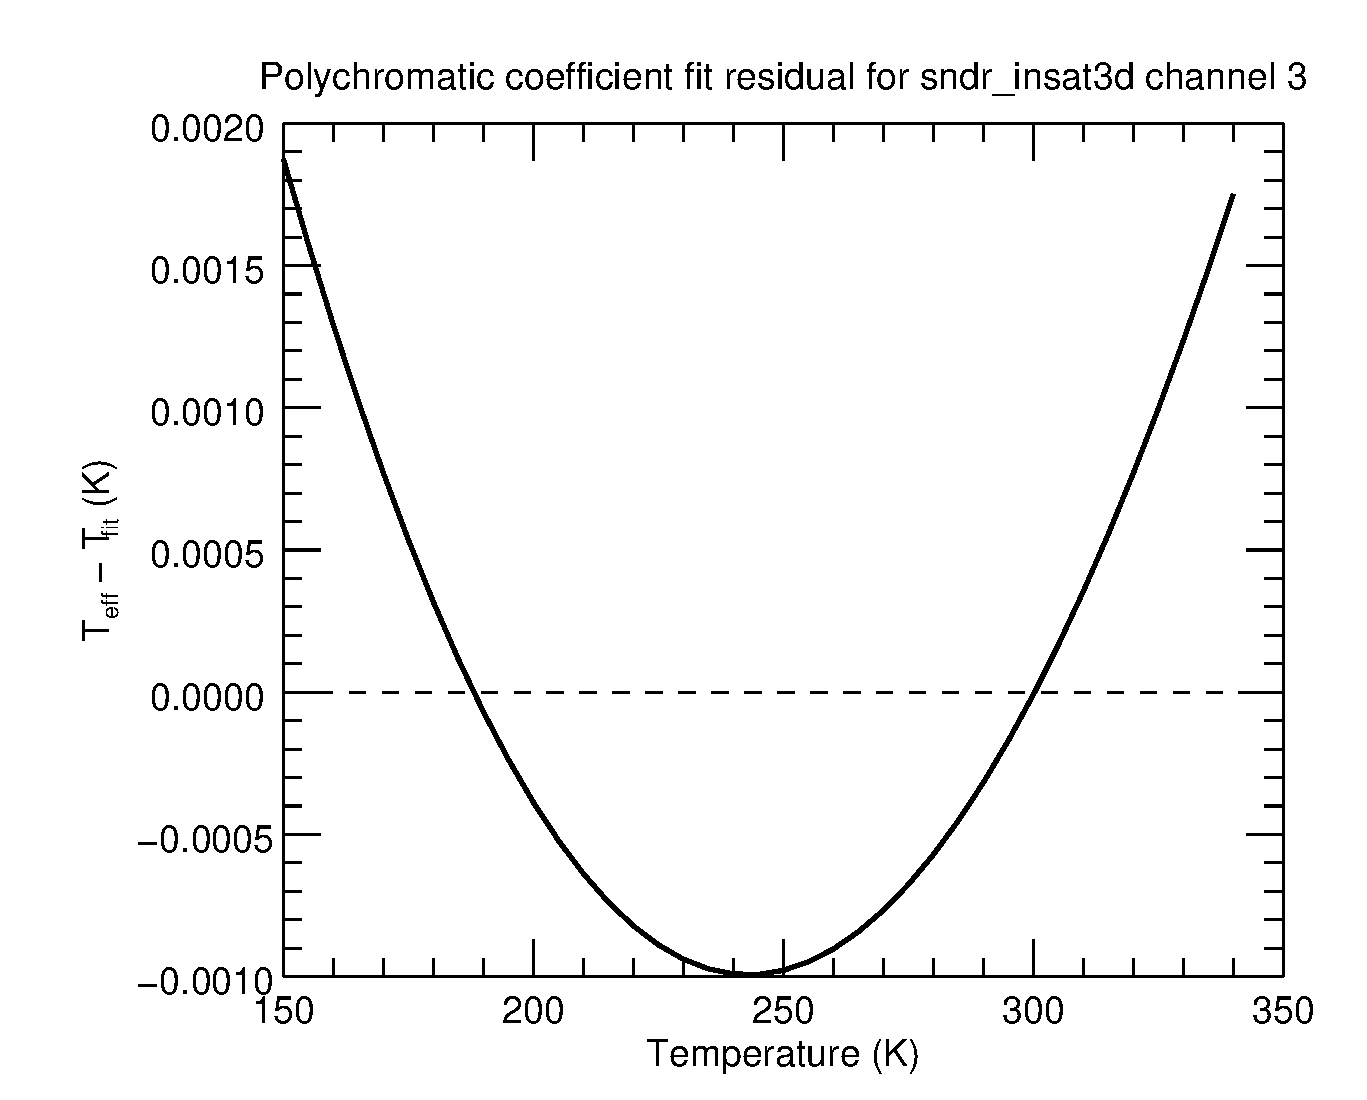
\includegraphics[scale=0.35]{graphics/sndr/tfit/sndr_insat3d-3.tfit.eps} &
    \includegraphics[scale=0.35]{graphics/sndr/tfit/sndr_insat3d-4.tfit.eps} \\\\
    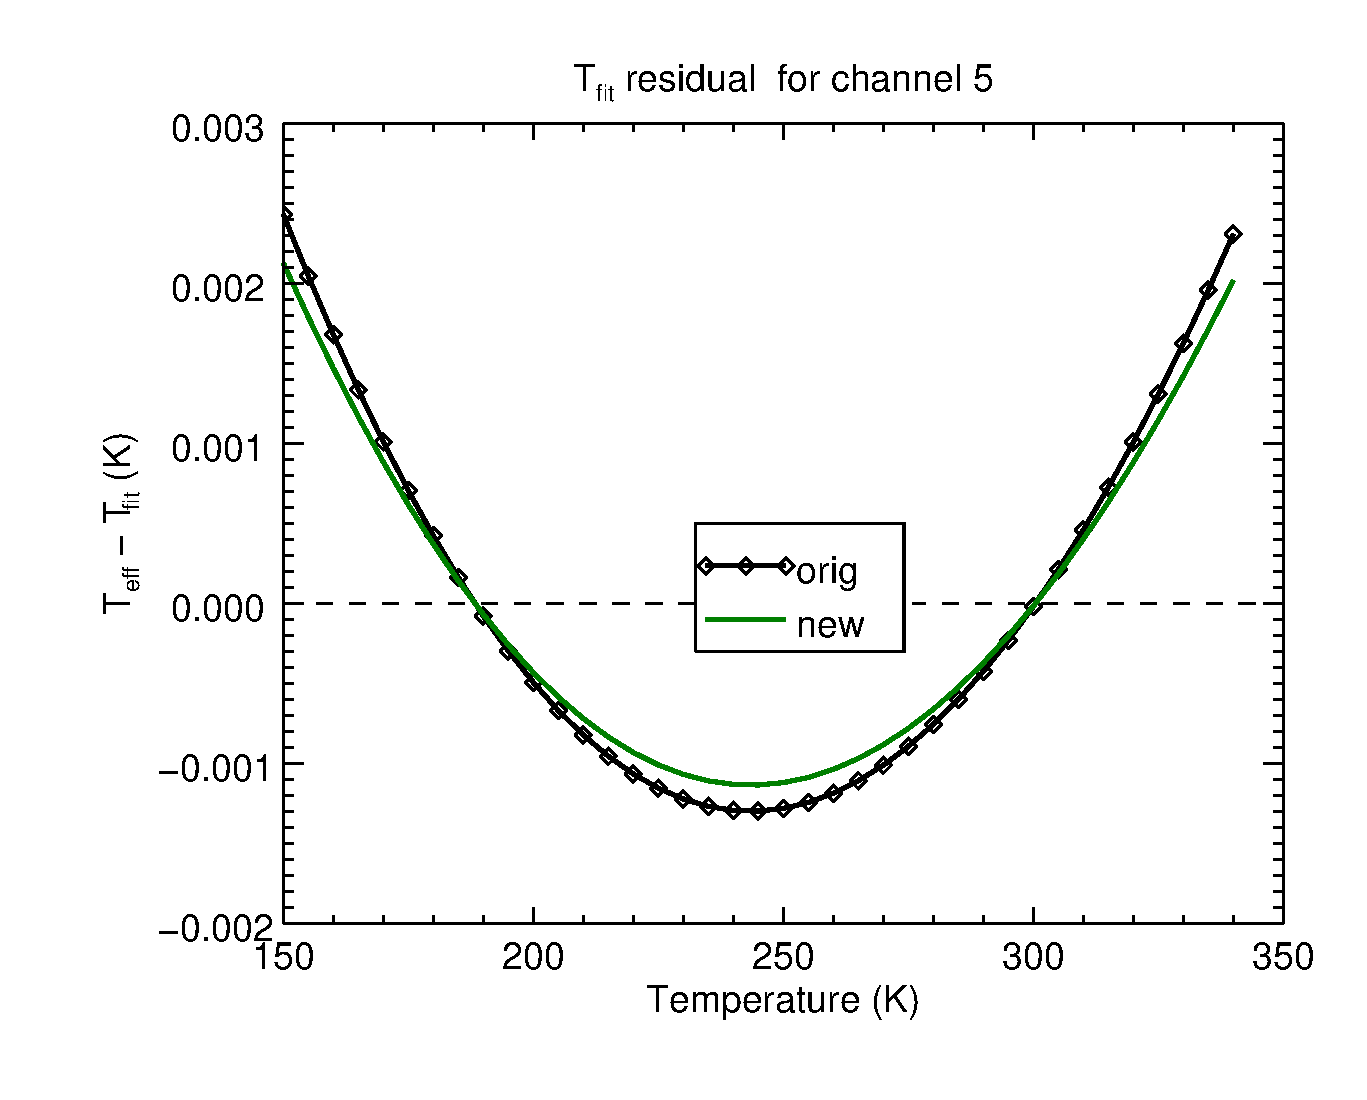
\includegraphics[scale=0.35]{graphics/sndr/tfit/sndr_insat3d-5.tfit.eps} &
    \includegraphics[scale=0.35]{graphics/sndr/tfit/sndr_insat3d-6.tfit.eps} \\
  \end{tabular}
  \caption{INSAT-3D Sounder channels 1-6 polychromatic correction temperature fit residuals.}
  \label{fig:sndr_ch1-6_tfit}
\end{figure}

\addcontentsline{toc}{subsubsection}{Channels 7-12}
\begin{figure}[H]
  \centering
  \begin{tabular}{c c}
    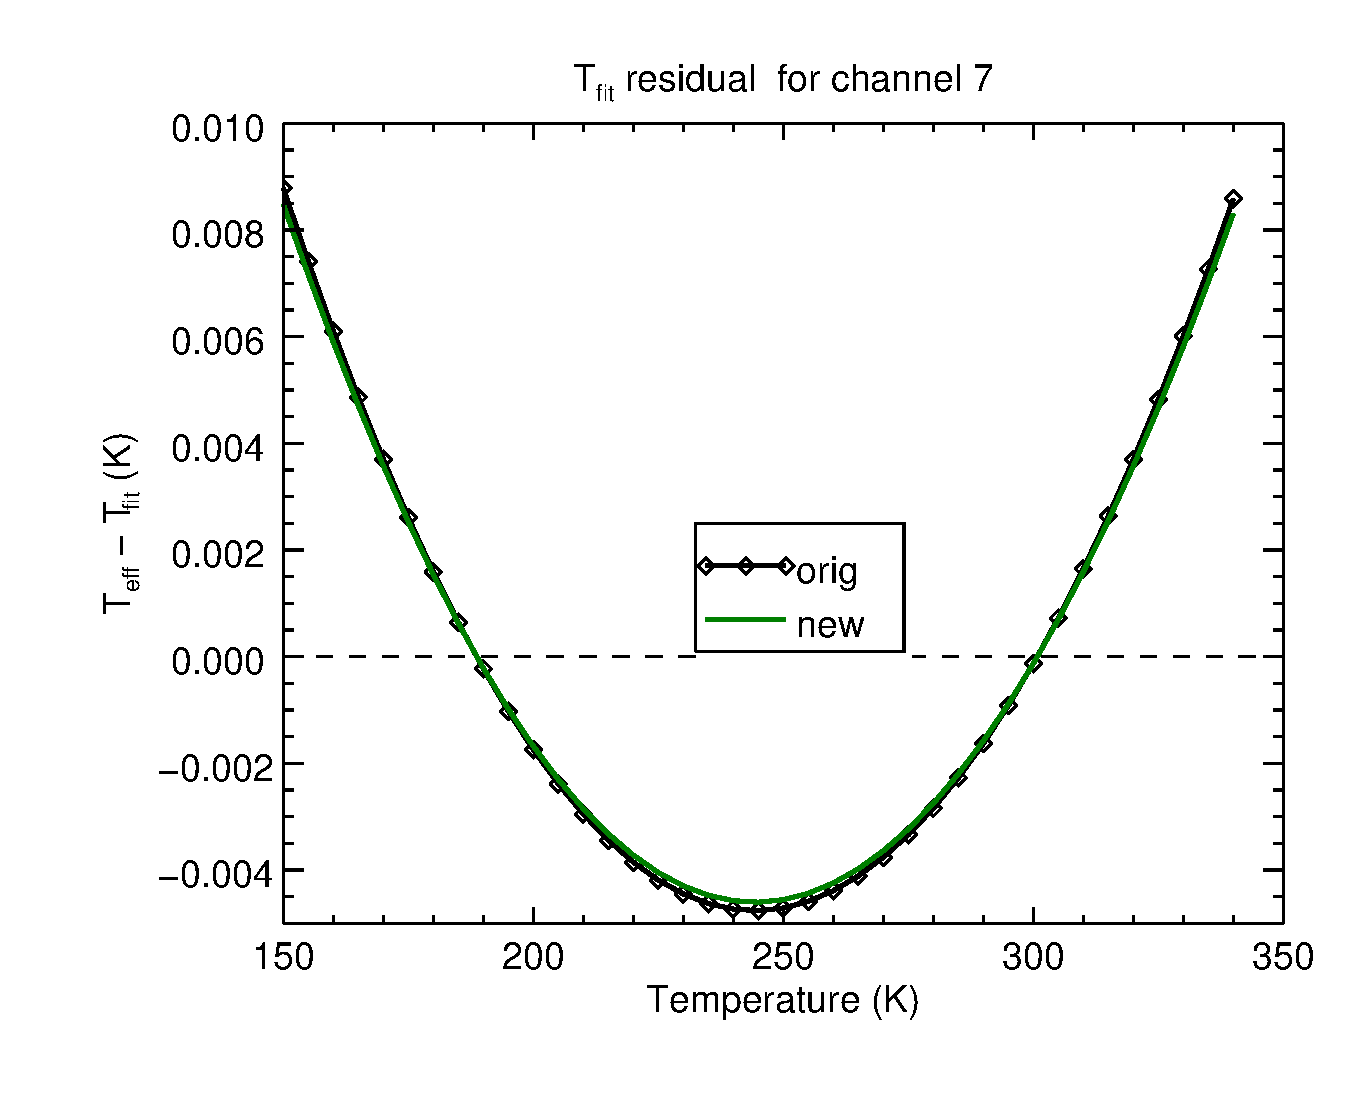
\includegraphics[scale=0.35]{graphics/sndr/tfit/sndr_insat3d-7.tfit.eps} &
    \includegraphics[scale=0.35]{graphics/sndr/tfit/sndr_insat3d-8.tfit.eps} \\\\
    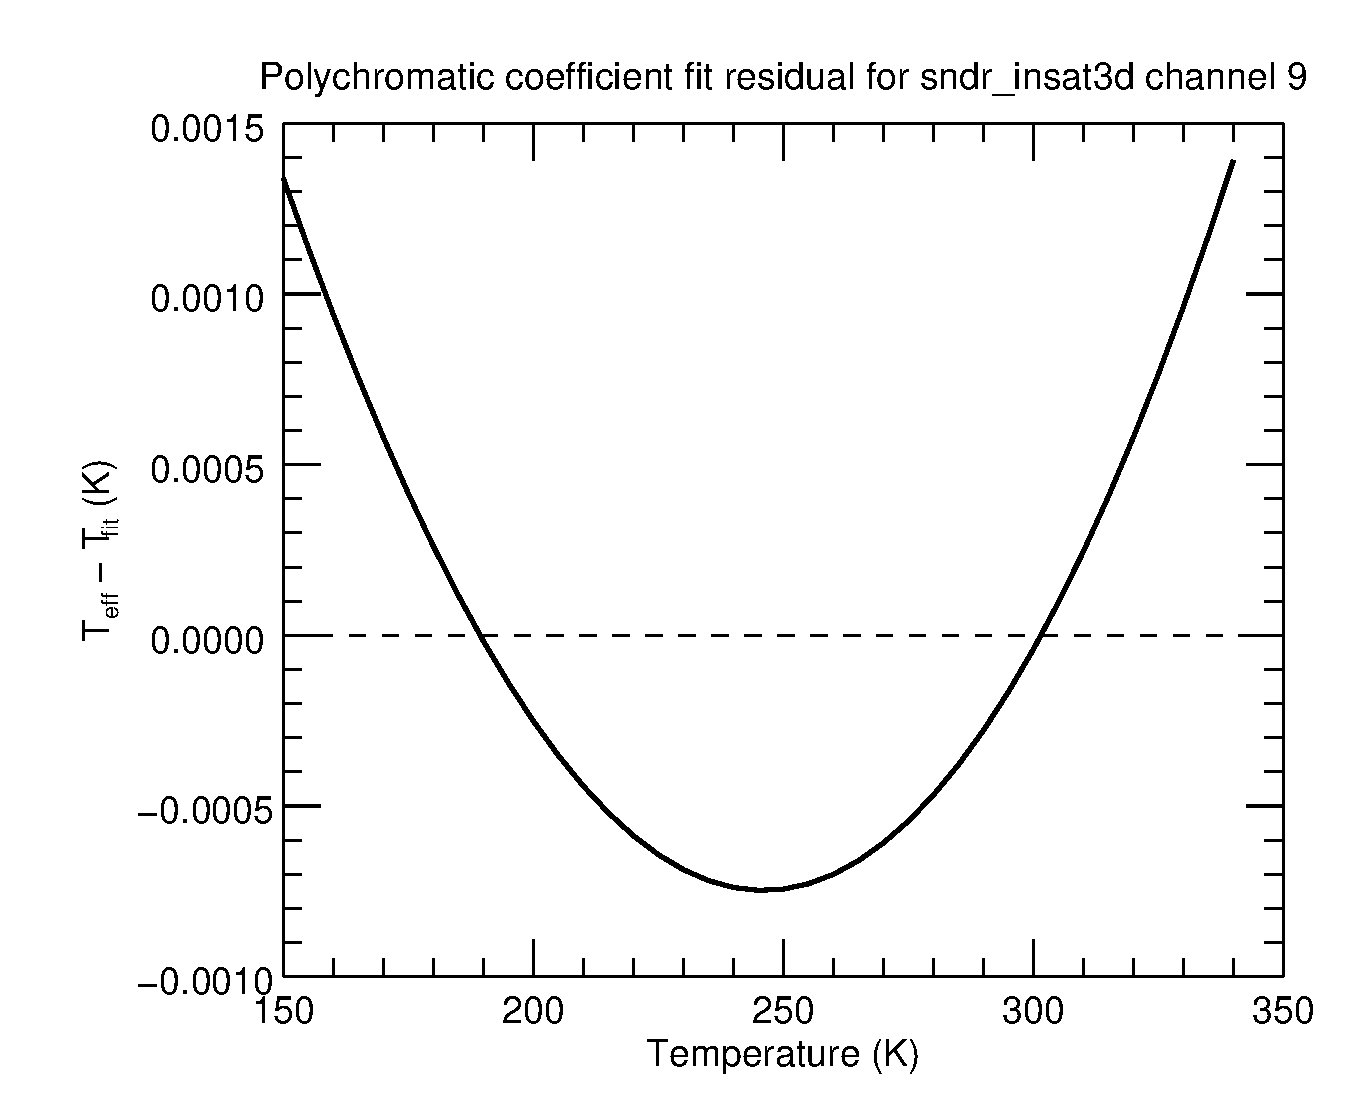
\includegraphics[scale=0.35]{graphics/sndr/tfit/sndr_insat3d-9.tfit.eps} &
    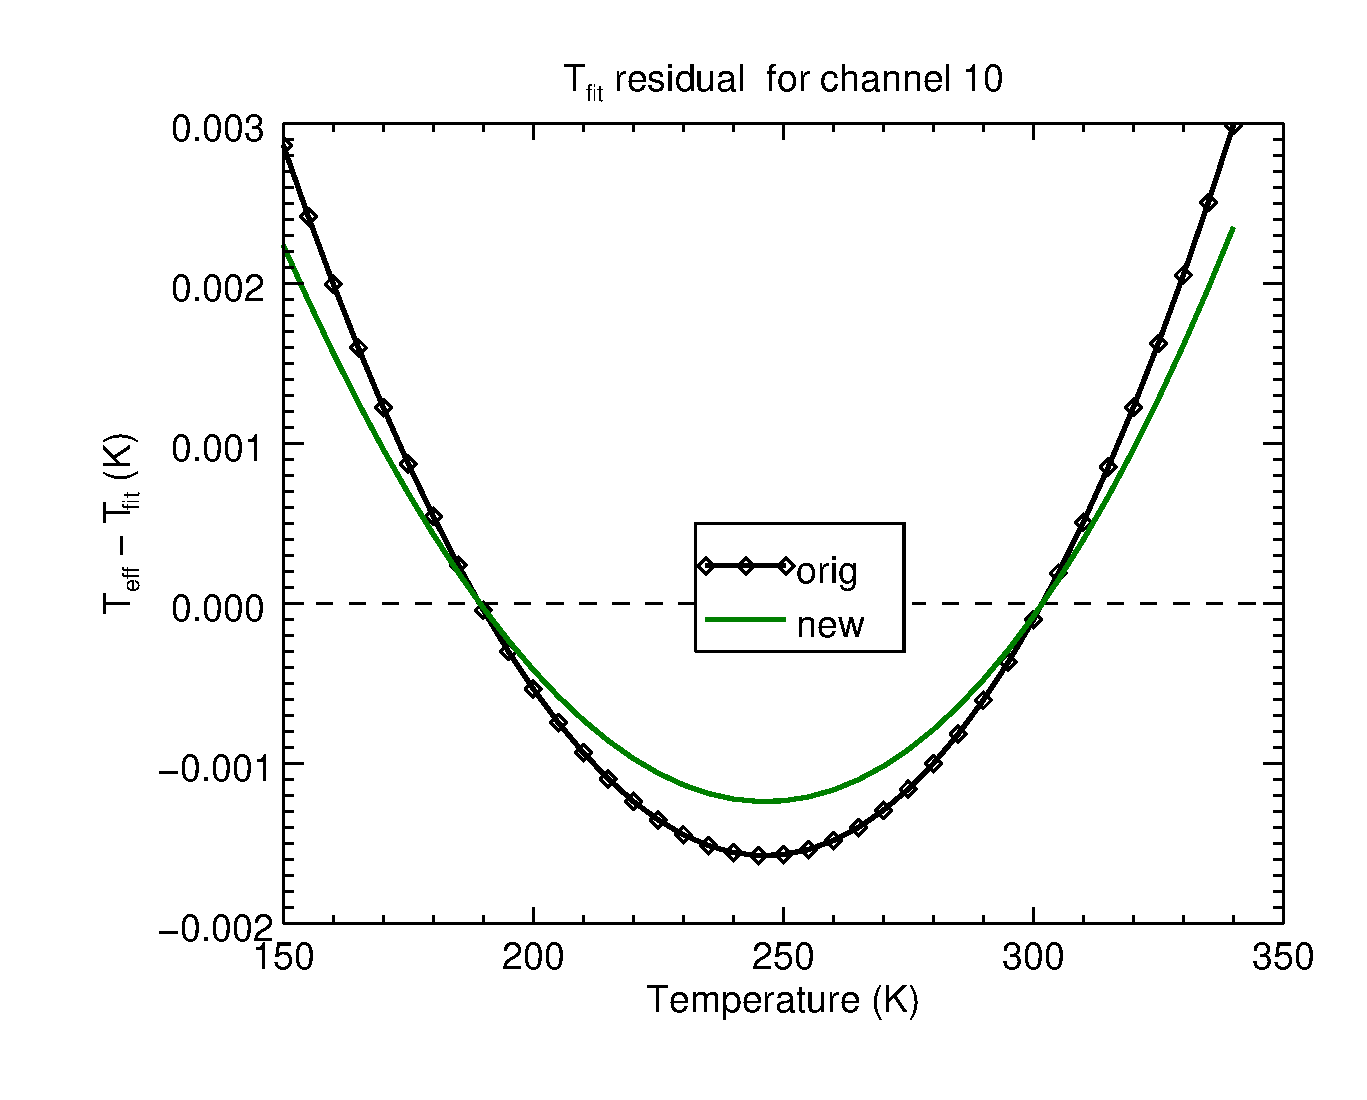
\includegraphics[scale=0.35]{graphics/sndr/tfit/sndr_insat3d-10.tfit.eps} \\\\
    \includegraphics[scale=0.35]{graphics/sndr/tfit/sndr_insat3d-11.tfit.eps} &
    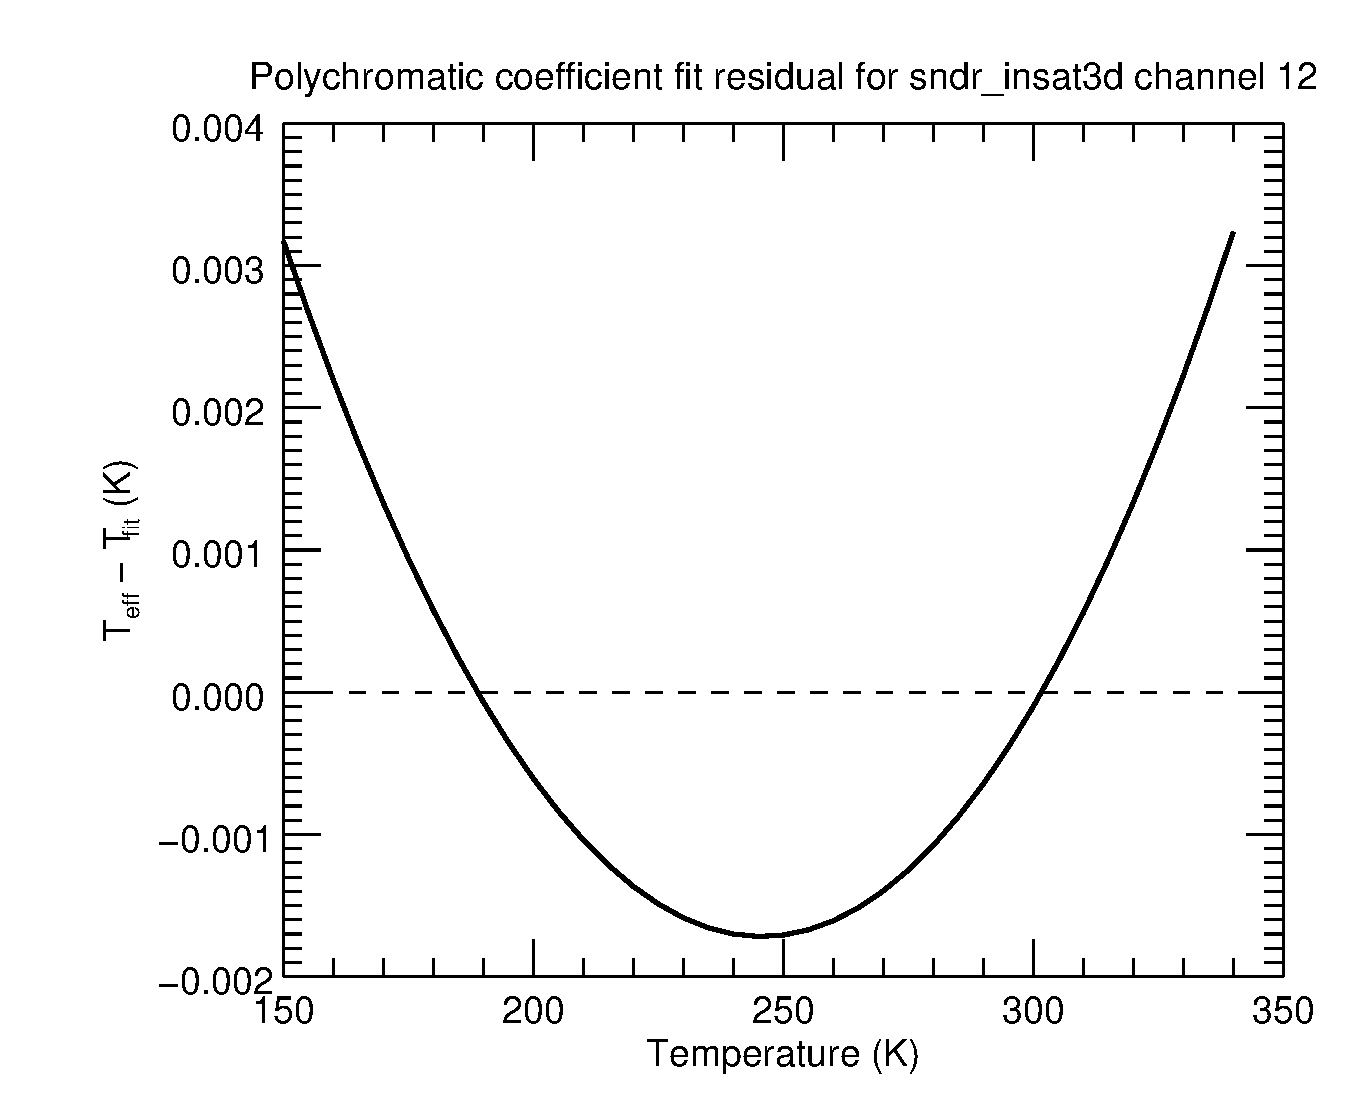
\includegraphics[scale=0.35]{graphics/sndr/tfit/sndr_insat3d-12.tfit.eps} \\
  \end{tabular}
  \caption{INSAT-3D Sounder channels 7-12 polychromatic correction temperature fit residuals.}
  \label{fig:sndr_ch7-12_tfit}
\end{figure}

\addcontentsline{toc}{subsubsection}{Channels 13-18}
\begin{figure}[H]
  \centering
  \begin{tabular}{c c}
    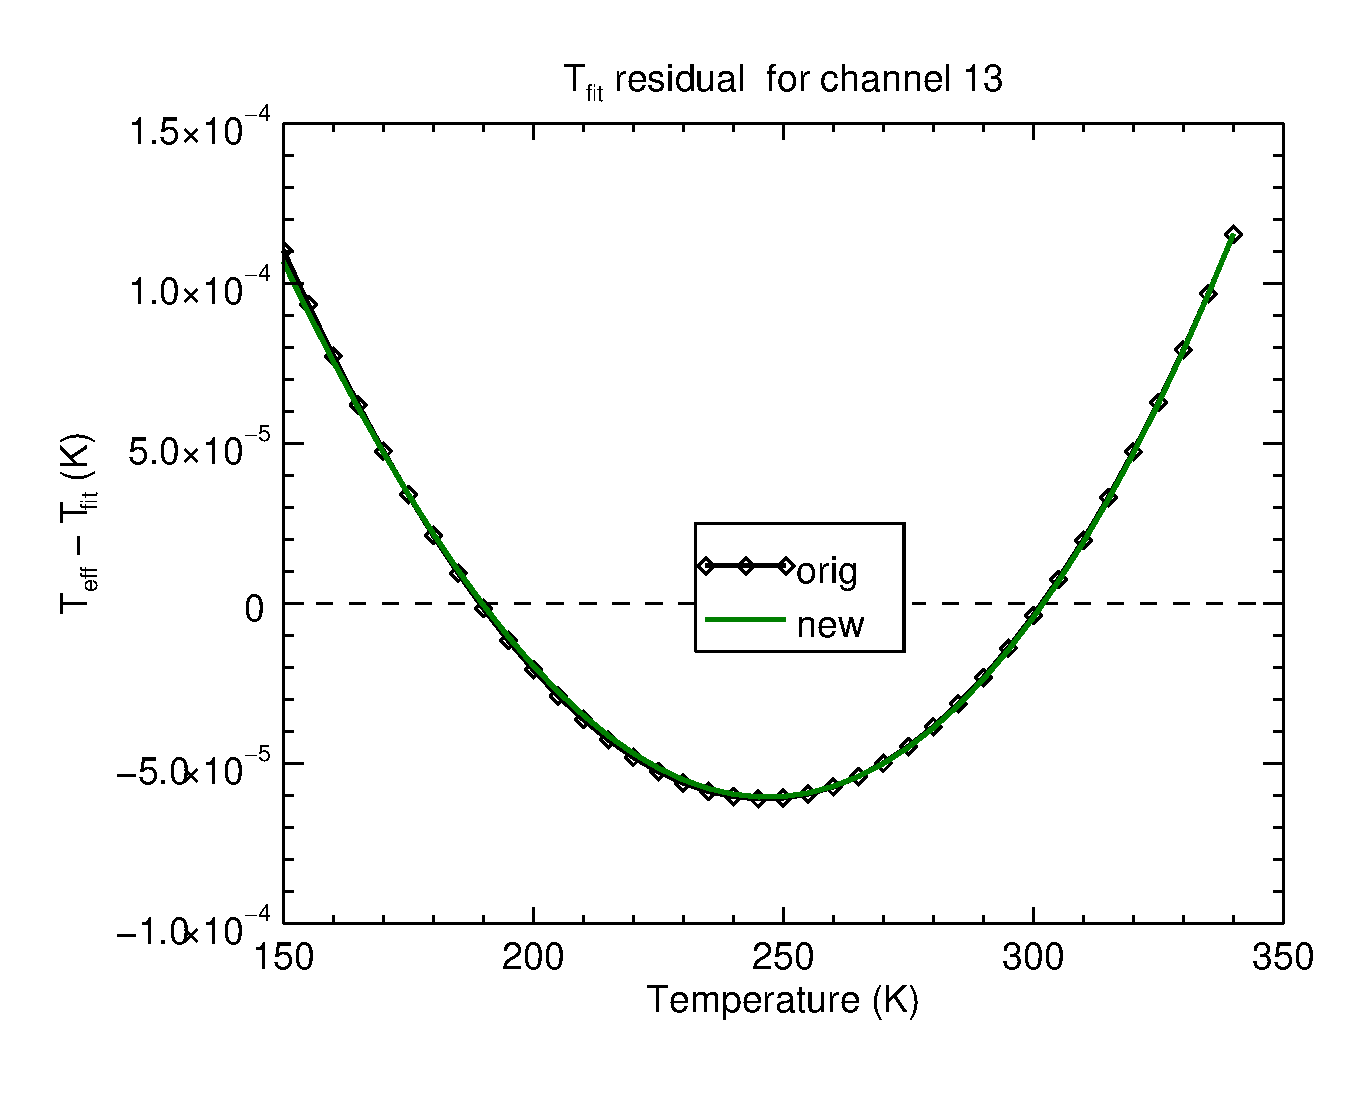
\includegraphics[scale=0.35]{graphics/sndr/tfit/sndr_insat3d-13.tfit.eps} &
    \includegraphics[scale=0.35]{graphics/sndr/tfit/sndr_insat3d-14.tfit.eps} \\\\
    \includegraphics[scale=0.35]{graphics/sndr/tfit/sndr_insat3d-15.tfit.eps} &
    \includegraphics[scale=0.35]{graphics/sndr/tfit/sndr_insat3d-16.tfit.eps} \\\\
    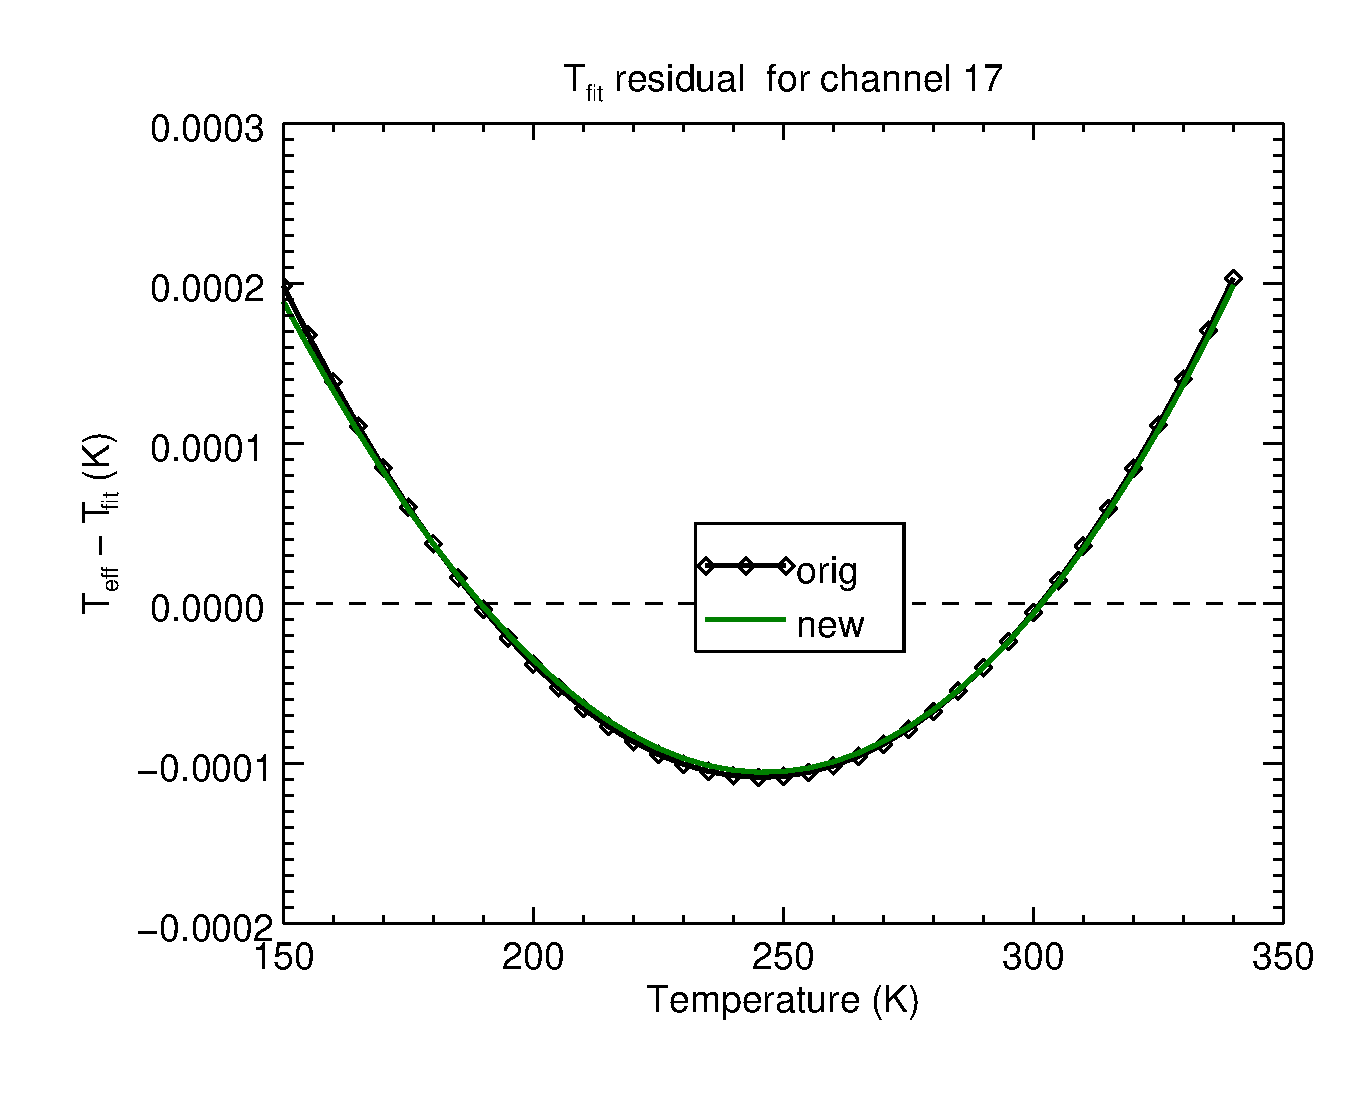
\includegraphics[scale=0.35]{graphics/sndr/tfit/sndr_insat3d-17.tfit.eps} &
    \includegraphics[scale=0.35]{graphics/sndr/tfit/sndr_insat3d-18.tfit.eps} \\
  \end{tabular}
  \caption{INSAT-3D Sounder channels 13-18 polychromatic correction temperature fit residuals.}
  \label{fig:sndr_ch13-18_tfit}
\end{figure}
